\part{Basic of Neural Networks and Verification}
\chapter{Basic of Neural Network}\label{sec:basic}

A \emph{neural network} (\textbf{NN})~\cite{Goodfellow-et-al-2016} consists of an input layer, multiple hidden layers, and an output layer. Each layer has a number of neurons, each connected to neurons in the next layer through a predefined set of weights (derived by training the network with data). A \emph{Deep Neural Network} (\textbf{DNN}) is an NN with two or more hidden layers. 

%A deep neural network consists of three types of layers: an input layer, multiple hidden layers, and an output layer. Each layer consists of a number of neurons, each connected to neurons from another layers through a predefined set of weights (derived by training the network with data). A network is called a \emph{fully connected feed-forward} neural network (FNN) if it connects every neuron in a layer (i.e., all weights are non-zero) to a neuron in the next layer.

The output of an NN is obtained by iteratively computing  the  values  of  neurons  in  each  layer.
The value of a neuron in the input layer is the input data. The value of a neuron in the hidden layers is computed by applying an \emph{affine transformation} (\autoref{sec:affine}) to values of neurons in the previous layers, then followed by an \emph{activation function} (\autoref{sec:activation}) such as ReLU and Sigmoid. The value of a neuron in the output layer is computed similarly but may skip the activation function.


%Fig.~\ref{fig:dnn}b shows the same network but with each hidden neuron $x$ split into two neurons $x'$ and $x''$ representing the result of affine transformation on $x$ and ReLU activation on $x'$, respectively, e.g.,  $x_3'=-x_1-0.5x_2-1.0$ and  $x_3'' = ReLU(x_3')$. This ReLU-slitting representation is adopted by \tool{} and other DNN analyses (e.g., ~\cite{katz2017reluplex,wang2018efficient,henriksen2020efficient}) 
% including Reluplex~\cite{katz2017reluplex}, Neurify~\cite{wang2018efficient}, and VeriNet~\cite{henriksen2020efficient},
%because it does not change the semantics or complexity of the problem and is easier to reason about as we will show in \S\ref{sec:overview}.

\section{Affine Transformation}\label{sec:affine}
The affine transformation (AF) of a neuron is the sum of the products of the weights of the incoming edges and the values of the neurons in the previous layer, plus the bias of the neuron.
More specifically, the AF of a neuron \(y\) with weights \(w_1, \dots, w_n\) and bias \(b\) and the values of neurons in the previous layer \(v_1, \dots, v_n\) is \(w_1v_1 + \dots + w_nv_n + b\). 

%AF is often applied to hidden layers of a DNN to compute the value of a neuron in the hidden layer.
%The values of a neuron in the output layer is evaluated similarly but it may skip the activation function.

For example, the AF of a neuron \(x_3\) in \autoref{fig:dnn} with (incoming arrows) weights \(-0.5, 0.5\) and bias \(1.0\) and the values of neurons in the previous layer \(x_1, x_2\) is \(-0.5x_1 + 0.5x_2 + 1.0\).

For DNN verification, AF is straightforward to reason about because it is a linear function. However, AFs are often followed by non-linear activation functions, described next in \autoref{sec:activation}, which make the verification problem more challenging.

\section{Activation Functions}\label{sec:activation}
Several popular activation functions used in DNNs include ReLU, Sigmoid, Tanh, and Softmax. All of these are non-linear\footnote{Non-linear means that the output of the function is not a linear combination of its inputs.} functions that introduce non-linearity to the network, allowing it to learn complex patterns in the data.


\begin{itemize}
\item ReLU (Rectified Linear Unit):  ReLU returns 0 if the input is less than zero, and the input itself otherwise. 
A ReLU activated neuron is said to be \emph{active} if its input value is greater than zero and \emph{inactive} otherwise.
ReLU is the most popular activation function in DNNs.\\
    \begin{center}
        $ReLU(x) = \max(x,0)$
    \end{center}


    
    
\item Sigmoid: Sigmoid is a smooth function that maps any real value to the range (0,1). It is often used in the output layer of a binary classification problem.\\
    \begin{center}
        $Sigmoid(x) = \frac{1}{1+e^{-x}}$
    \end{center}
\item Tanh: Tanh is similar to the sigmoid function but maps any real value to the range (-1,1). It is often used in the output layer of a multi-class classification problem.\\
    \begin{center}
        $Tanh(x) = \frac{e^x-e^{-x}}{e^x+e^{-x}}$
    \end{center}
\item Softmax: Softmax is a generalization of the sigmoid function that maps any real value to the range (0,1) and ensures that the sum of the output values is 1. It is often used in the output layer of a multi-class classification problem.\\
    \begin{center}
    $Softmax(x)_i = \frac{e^{x_i}}{\sum_{j=1}^{n}e^{x_j}}$
    \end{center}
\end{itemize}

For DNN verification, these non-linear activation functions make verification difficult because it introduces multiple possible outcomes for any input, making it hard to reason about the output of the network. For example, ReLU has two possible outputs for any input: 0 if the input is less than zero, and the input itself otherwise, and Sigmoid has a smooth curve with infinite possible outputs for any input.


\section{Example} 
Fig.~\ref{fig:dnn} shows a simple DNN with two inputs $x_1,x_2$, two hidden neurons $x_3,x_4$, and one output $x_5$. The weights of a neuron are shown on its incoming edges, and the bias is shown above or below each neuron. The outputs of the hidden neurons  are computed the affine transformation and ReLU, e.g., $x_3 = ReLU(-0.5x_1+0.5x_2+1.0)$. The output neuron is computed with just the affine transformation, i.e., $x_5=-x_3+x_4-1$.


\begin{figure}
    \centering
    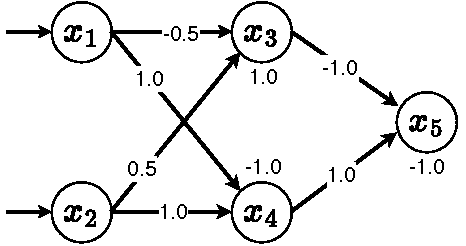
\includegraphics[width=0.5\linewidth]{figure/dnn.pdf}
    \caption{\label{fig:dnn} An FNN with ReLU.}
\end{figure}


\section{Types of Neural Networks}


\paragraph{Feed-Forward Network (FFN)} In an FFN information flows in one direction, from the input layer to hidden layers to the output layer (and thus no cycle).  

A fully connected feed-forward neural network (FNN), shown below, is an FFN where every neuron in a layer is connected to every neuron in the next layer.
\begin{center}
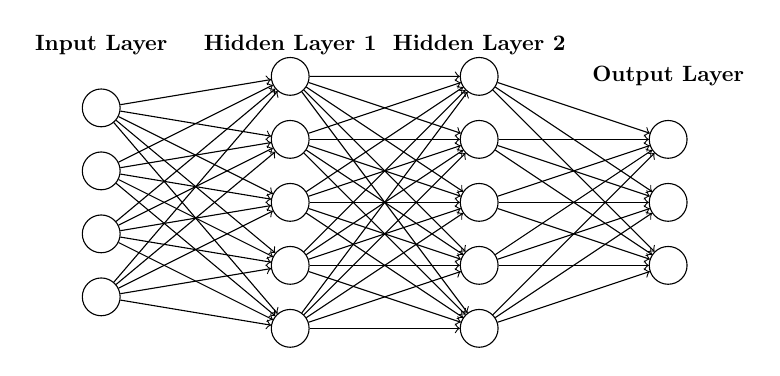
\begin{tikzpicture}[scale=0.8, transform shape]
% Input Layer
\node at (0,4) {\textbf{Input Layer}};
\foreach \x in {1,2,3,4} {
    \node[circle, draw=black, fill=white, minimum size=0.6cm] (I\x) at (0,4-\x) {};
}

% Hidden Layer 1
\node at (3,4) {\textbf{Hidden Layer 1}};
\foreach \x in {1,2,3,4,5} {
    \node[circle, draw=black, fill=white, minimum size=0.6cm] (H1\x) at (3,4.5-\x) {};
}

% Hidden Layer 2
\node at (6,4) {\textbf{Hidden Layer 2}};
\foreach \x in {1,2,3,4,5} {
    \node[circle, draw=black, fill=white, minimum size=0.6cm] (H2\x) at (6,4.5-\x) {};
}

% Output Layer
\node at (9,3.5) {\textbf{Output Layer}};
\foreach \x in {1,2,3} {
    \node[circle, draw=black, fill=white, minimum size=0.6cm] (O\x) at (9,3.5-\x) {};
}

% Connections
\foreach \i in {1,2,3,4}
    \foreach \j in {1,2,3,4,5}
        \draw[->] (I\i) -- (H1\j);

\foreach \i in {1,2,3,4,5}
    \foreach \j in {1,2,3,4,5}
        \draw[->] (H1\i) -- (H2\j);

\foreach \i in {1,2,3,4,5}
    \foreach \j in {1,2,3}
        \draw[->] (H2\i) -- (O\j);

\end{tikzpicture}
\end{center}





\paragraph{Convolutional Neural Networks (CNNs)} CNNs, often used in image recognition and classification, consist of neurons that have learnable weights and biases. Each neuron receives several inputs, takes a weighted sum over them, passes it through an activation function, and responds with an output.

\paragraph{Recurrent Neural Networks (RNNs)} RNNs, often used in natural language process and speech recognition, are designed to recognize patterns in sequences of data. RNNs have \emph{loops} in them, allowing information to be sent forward and backward.

\paragraph{Residual Networks} Residual Networks (ResNets) are a type of neural network that is often used in image recognition and classification. ResNets introduce skip connections that allow the gradient to flow directly through the network, making it easier to train deep networks.

\section{Properties of Neural Networks}
Similar to software programs, neural networks have desirable properties to ensure the network behaves as expected. These could be specific to the applications modeled by the network, e.g., safety properties in a collision avoidance system or general properties that are desired by all networks, e.g., robustness to adversarial attacks. 


\paragraph{Robustness Properties}
\emph{Robustness}, a desirable property for all networks, ensures that small perturbations in the input data do not cause major changes in the output of the network. For example, if a few pixels in an image are changed, the network should still classify the image correctly. \emph{Adversarial attacks} are a common way to test the robustness of a neural network. In an adversarial attack, an attacker makes small changes to the input data to cause the network to misclassify the data.

\emph{Local} robustness refers to robustness of a neural network within a \emph{small neighborhood or region} of the input data. In contrast, \emph{global} robustness refers to robustness of a network across the \emph{entire input space}. Global robustness is harder to achieve than local robustness, as it requires the network to be robust to all possible inputs.

\paragraph{$\epsilon$-robustness} A neural network is $\epsilon$-robust if the difference between any two inputs $x$ and $x'$ is within a small range $\epsilon$, the output $f$ of the network does not change significantly (or remain the same), i.e., $\|x-x'\| \leq \epsilon \implies f(x) \approx f(x')$.




\paragraph{Safety Properties} Safety properties are specific to the application modeled by the network. For example, a safety property in a collision avoidance system might be that if the intruder is distant and significantly slower than us, then we stay below a certain threshold, i.e., $d_{intruder} > d_{threshold} \land v_{intruder} < v_{threshold} \implies v_{us} < v_{threshold}$.


\subsection{Challenges}

\paragraph{Formalization}


\paragraph{Expressiveness}




\chapter{Verification of Neural Networks}\label{sec:verification}


\section{The Neural Network Verification (NNV) Problem}\label{sec:nnv-problem}
\paragraph{DNN Verification} Given a DNN \(N\) and a property $\phi$, the \emph{DNN verification problem} asks if $\phi$ is a valid property of $N$.
Typically, $\phi$ is a formula of the form $\phi_{in} \Rightarrow \phi_{out}$, where $\phi_{in}$ is a property over the inputs of $N$ and $\phi_{out}$ is a property over the outputs of $N$.
%This form of properties has been used to encode safety and security requirements of DNNs, e.g., safety specifications to avoid collision in unmanned aircraft~\cite{kochenderfer2012next} and \emph{adversarial robustness}~\cite{katz2017towards} properties desired by all DNNs, in which a small input perturbation does not cause major spikes in the DNN's outputs.
A DNN verifier attempts to find a \emph{counterexample} input to $N$ that satisfies $\phi_{in}$ but violates $\phi_{out}$.  If no such counterexample exists, $\phi$ is a valid property of $N$. Otherwise, $\phi$ is not valid and the counterexample can be used to retrain or debug the DNN~\cite{huang2017safety}.




% Verification tool such as Marabou and nnenum are then applied to the network to prove that the network is safe or identifier counterexample representing small input differences causing large output changes.


% \footnote{This is encoded as the differences of the inputs being within a certain small range  ($\phi_{in}$) implies the differences of the outputs still fall within a certain range in $\phi_{out}$)}.



\paragraph{Example} A valid property for the DNN in \autoref{fig:dnn} is that the output is $x_5 \le 0$ for any inputs $x_1 \in [-1,1], x_2\in[-2,2]$. An invalid property is that $x_5 > 0$ for those similar inputs.
A counterexample showing this property violation is $\{x_1=-1, x_2=2\}$, from which the DNN evaluates to $x_5=-3.5$. 

%Such properties can capture \emph{safety requirements} (e.g., a rule in an  collision avoidance system in~\cite{kochenderfer2012next,katz2017reluplex} is ``if the intruder is distant and significantly slower than us, then we stay below a certain threshold'') or \emph{local robustness}~\cite{katz2017towards} conditions (a form of adversarial robustness stating that small perturbations of a given input all yield the same output).


\section{Satisfiability and Activation Pattern Search}\label{sec:satisfiability-and-activation-pattern-search}

 As with traditional software, DNN verification is often represented as a satisfiability problem.
We thus need to define a formula to represent the network. Typically this formula is a conjunction of constraints representing the affine transformation and activation function of each neuron in the network.
For a network with $L$ layers, $N$ neurons per layer, and ReLU activations this formula is:
\begin{align*}
\alpha = \bigwedge_{\begin{smallmatrix}i \in [1,L]\\ j \in [1,N]\end{smallmatrix}} v_{i,j} = \max \Big( \sum_{k \in [1,N]} (w_{i-1,j,k} \cdot v_{i-1,j}) + b_{i,j}, 0 \Big)
\end{align*}
With this definition DNN verification can be formulated as checking the satisfiability of:
\begin{equation}\label{eq:prob}
  \alpha \land \phi_{in} \land \neg \phi_{out}
\end{equation}
If \autoref{eq:prob} is unsatisfiable, $\phi$ is a valid property of $\mathcal{N}$. Otherwise, $\phi$ is not valid (and the counterexample of the original problem is any satisfying assignment that makes \autoref{eq:prob} true).


\section{Activation Pattern Search} For the widely-used ReLU activation problem, the DNN verification problem becomes a search for \emph{activation patterns}, i.e., boolean assignments representing activation status of neurons, that lead to satisfaction the formula in \autoref{eq:prob}. 

Modern DNN verification techniques~\cite{bunel2020branch,wang2021beta,ferrari2022complete,duong2024harnessing,duong2023dpllt,ovalbab,katz2019marabou,bak2021nnenum} all adopt this idea and search for satisfying activation patterns.


\section{Complexity}

